\documentclass[12pt]{article}
\usepackage{amsmath}
\usepackage{amsfonts}
\usepackage{amssymb}
\usepackage{graphicx}
\usepackage[a4paper, margin=0.98in]{geometry}
\usepackage{physics}
\usepackage{float}
\usepackage{booktabs}
\usepackage{makecell}
\usepackage{helvet}
\usepackage{fancyhdr}
\usepackage{titling}
\usepackage{longtable}
\usepackage{caption}
\usepackage{enumitem}
\usepackage{circuitikz}
\usepackage[hidelinks]{hyperref}
\usepackage{tikz}



% Define header
\pagestyle{fancy}
\fancyhf{}
\fancyhead[R]{PH3204: Electronics Laboratory}

% Title
\title{
  \vspace{-2cm}
  \Huge \textbf{PH3204: Electronics Laboratory} \\[0.4cm]
  \Large \textbf{Experiment 03:  Study of Operational Amplifier 
  (OpAmp) as inverting and non-inverting amplifier and
  its applications as adder and subtractor}
}

\author{
  \textbf{Ronit Bhuyan (22MS025)} \\[0.2cm]
  \textbf{Sub-Group B01}
}

\date{\today}

\begin{document}

\maketitle

\tableofcontents
\noindent\rule{\textwidth}{0.4pt}
\newpage

\section{Theory}


\subsection{Operational Amplifier (OpAmp)}
An Operational Amplifier or OpAmp is a differential amplifier that has a very high voltage gain, high input impedance and low output impedance. The OpAmp ha two inputs namely a non-inverting input($V_+$) and an inverting input($V_-$). The OpAmp amplifies the difference between the two inputs. The output voltage ($V_{out}$) is given by 
\begin{align*}
    V_{out} = A(V_+ - V_-)
\end{align*} 
where $A$ is the open loop gain of the amplifier. The OpAmp is usually operated with a negative feedback. The OpAmp used in this experiment is the LM741 OpAmp. The pin configuration of the LM741 OpAmp and its circuit diagram is shown in the figure below.




\begin{figure}[H]
\centering
\begin{minipage}{0.25\textwidth}
\centering
  



\tikzset{every picture/.style={line width=0.75pt}} %set default line width to 0.75pt        

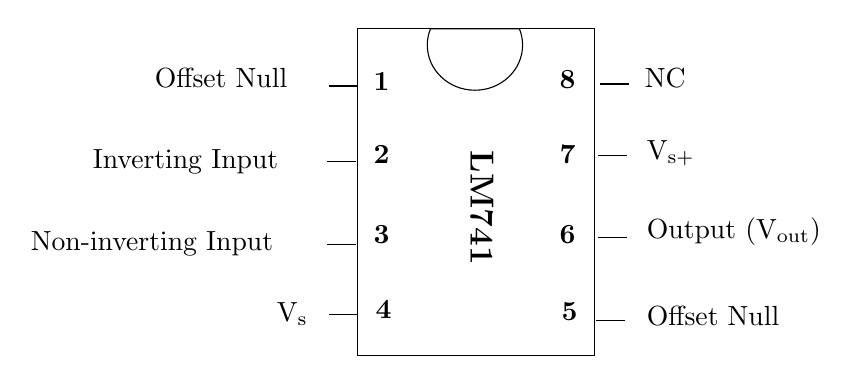
\begin{tikzpicture}[x=0.70pt,y=0.70pt,yscale=-1,xscale=1]
%uncomment if require: \path (0,300); %set diagram left start at 0, and has height of 300

%Shape: Rectangle [id:dp7033944784081119] 
\draw   (229,50.6) -- (351.2,50.6) -- (351.2,219.4) -- (229,219.4) -- cycle ;
%Shape: Chord [id:dp3994312770777564] 
\draw   (312.57,50.94) .. controls (313.62,53.53) and (314.2,56.35) .. (314.2,59.3) .. controls (314.2,72.17) and (303.19,82.6) .. (289.6,82.6) .. controls (276.01,82.6) and (265,72.17) .. (265,59.3) .. controls (265,56.35) and (265.58,53.53) .. (266.63,50.94) -- cycle ;
%Straight Lines [id:da12448979123953197] 
\draw    (214.2,80.4) -- (229.2,80.4) ;
%Straight Lines [id:da32433624264635386] 
\draw    (354.2,79.4) -- (369.2,79.4) ;
%Straight Lines [id:da4099130005520506] 
\draw    (214.2,198.4) -- (229.2,198.4) ;
%Straight Lines [id:da5527837141478477] 
\draw    (213.2,162.4) -- (228.2,162.4) ;
%Straight Lines [id:da7926452153091902] 
\draw    (213.2,119.4) -- (219.2,119.4) -- (228.2,119.4) ;
%Straight Lines [id:da3175360193460135] 
\draw    (352.2,201.4) -- (367.2,201.4) ;
%Straight Lines [id:da18341325604541547] 
\draw    (353.2,158.4) -- (368.2,158.4) ;
%Straight Lines [id:da46969219793073524] 
\draw    (353.2,116.4) -- (368.2,116.4) ;

% Text Node
\draw (300.5,112.5) node [anchor=north west][inner sep=0.75pt]  [rotate=-90] [align=left] {\textbf{{\large LM741}}};
% Text Node
\draw (236,72) node [anchor=north west][inner sep=0.75pt]   [align=left] {\textbf{1}};
% Text Node
\draw (237,190) node [anchor=north west][inner sep=0.75pt]   [align=left] {\textbf{4}};
% Text Node
\draw (236,151) node [anchor=north west][inner sep=0.75pt]   [align=left] {\textbf{3}};
% Text Node
\draw (236,110) node [anchor=north west][inner sep=0.75pt]   [align=left] {\textbf{2}};
% Text Node
\draw (333,191) node [anchor=north west][inner sep=0.75pt]   [align=left] {\textbf{5}};
% Text Node
\draw (332,151) node [anchor=north west][inner sep=0.75pt]   [align=left] {\textbf{6}};
% Text Node
\draw (332,110) node [anchor=north west][inner sep=0.75pt]   [align=left] {\textbf{7}};
% Text Node
\draw (332,71) node [anchor=north west][inner sep=0.75pt]   [align=left] {\textbf{8}};
% Text Node
\draw (123,70) node [anchor=north west][inner sep=0.75pt]   [align=left] {Offset Null};
% Text Node
\draw (91,112) node [anchor=north west][inner sep=0.75pt]   [align=left] {Inverting Input};
% Text Node
\draw (59,154) node [anchor=north west][inner sep=0.75pt]   [align=left] {Non-inverting Input};
% Text Node
\draw (90,189) node [anchor=north west][inner sep=0.75pt]   [align=left] {$ $};
% Text Node
\draw (186,191) node [anchor=north west][inner sep=0.75pt]   [align=left] {$\mathrm{V_{s}}$};
% Text Node
\draw (376,70) node [anchor=north west][inner sep=0.75pt]   [align=left] {NC};
% Text Node
\draw (377,107) node [anchor=north west][inner sep=0.75pt]   [align=left] {$\mathrm{V_{s+}}$};
% Text Node
\draw (377,150) node [anchor=north west][inner sep=0.75pt]   [align=left] {$ $};
% Text Node
\draw (377,147) node [anchor=north west][inner sep=0.75pt]   [align=left] {Output ($\mathrm{V_{out}})$};
% Text Node
\draw (377,193) node [anchor=north west][inner sep=0.75pt]   [align=left] {Offset Null};


\end{tikzpicture}

\end{minipage}
\hfill
\begin{minipage}{0.30\textwidth}
\centering






\tikzset{every picture/.style={line width=0.75pt}} %set default line width to 0.75pt        

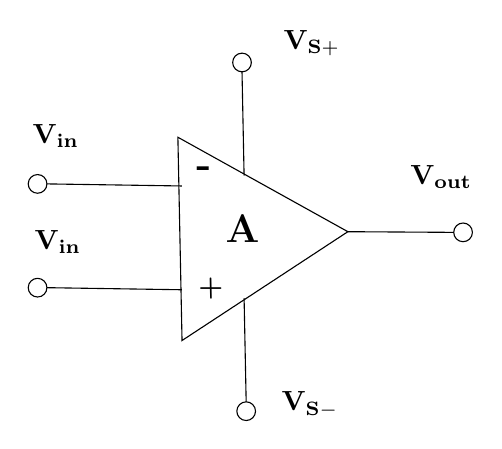
\begin{tikzpicture}[x=0.75pt,y=0.75pt,yscale=-1,xscale=1]
%uncomment if require: \path (0,300); %set diagram left start at 0, and has height of 300

%Flowchart: Extract [id:dp37966680550104925] 
\draw   (342.2,127.03) -- (262.3,179.46) -- (260.3,81.52) -- cycle ;
%Straight Lines [id:da7450651132831247] 
\draw    (197.2,104) -- (262.2,105) ;
%Straight Lines [id:da22744928578481094] 
\draw    (197.2,154) -- (262.2,155) ;
%Straight Lines [id:da9998583755076631] 
\draw    (342.2,127.03) -- (393.2,127.35) ;
%Straight Lines [id:da5159377376383624] 
\draw    (291.2,50) -- (292.2,100) ;
%Straight Lines [id:da38245740821617125] 
\draw    (292.2,159) -- (293.2,209) ;
%Shape: Circle [id:dp7432178640178844] 
\draw   (286.7,45.5) .. controls (286.7,43.01) and (288.71,41) .. (291.2,41) .. controls (293.69,41) and (295.7,43.01) .. (295.7,45.5) .. controls (295.7,47.99) and (293.69,50) .. (291.2,50) .. controls (288.71,50) and (286.7,47.99) .. (286.7,45.5) -- cycle ;
%Shape: Circle [id:dp8582173243755384] 
\draw   (288.7,213.5) .. controls (288.7,211.01) and (290.71,209) .. (293.2,209) .. controls (295.69,209) and (297.7,211.01) .. (297.7,213.5) .. controls (297.7,215.99) and (295.69,218) .. (293.2,218) .. controls (290.71,218) and (288.7,215.99) .. (288.7,213.5) -- cycle ;
%Shape: Circle [id:dp6580404394197098] 
\draw   (188.2,104) .. controls (188.2,101.51) and (190.21,99.5) .. (192.7,99.5) .. controls (195.19,99.5) and (197.2,101.51) .. (197.2,104) .. controls (197.2,106.49) and (195.19,108.5) .. (192.7,108.5) .. controls (190.21,108.5) and (188.2,106.49) .. (188.2,104) -- cycle ;
%Shape: Circle [id:dp4152539024478965] 
\draw   (188.2,154) .. controls (188.2,151.51) and (190.21,149.5) .. (192.7,149.5) .. controls (195.19,149.5) and (197.2,151.51) .. (197.2,154) .. controls (197.2,156.49) and (195.19,158.5) .. (192.7,158.5) .. controls (190.21,158.5) and (188.2,156.49) .. (188.2,154) -- cycle ;
%Shape: Circle [id:dp8877611769090077] 
\draw   (393.2,127.35) .. controls (393.2,124.86) and (395.21,122.85) .. (397.7,122.85) .. controls (400.19,122.85) and (402.2,124.86) .. (402.2,127.35) .. controls (402.2,129.84) and (400.19,131.85) .. (397.7,131.85) .. controls (395.21,131.85) and (393.2,129.84) .. (393.2,127.35) -- cycle ;

% Text Node
\draw (282,118) node [anchor=north west][inner sep=0.75pt]   [align=left] {\textbf{{\Large A}}};
% Text Node
\draw (189,74) node [anchor=north west][inner sep=0.75pt]   [align=left] {$\mathbf{V_{in}}$};
% Text Node
\draw (190,125) node [anchor=north west][inner sep=0.75pt]   [align=left] {$\mathbf{V_{in}}$};
% Text Node
\draw (371,94) node [anchor=north west][inner sep=0.75pt]   [align=left] {$\mathbf{V_{out}}$};
% Text Node
\draw (310,29) node [anchor=north west][inner sep=0.75pt]   [align=left] {$\mathbf{V_{S+}}$};
% Text Node
\draw (309,203) node [anchor=north west][inner sep=0.75pt]   [align=left] {$\mathbf{V_{S-}}$};
% Text Node
\draw (268,91) node [anchor=north west][inner sep=0.75pt]   [align=left] {\textbf{{\Large -}}};
% Text Node
\draw (268.85,148) node [anchor=north west][inner sep=0.75pt]  [xslant=-0.02] [align=left] {\textbf{+}};


\end{tikzpicture}

\end{minipage}
\\
\caption{\centering Pin configuration of LM741 OPAMP (left) and its circuit symbol (right)}
\end{figure}
\noindent
The OpAmp can be used in various configurations such as inverting amplifier, non-inverting amplifier, adder, subtractor,differentiator, integrator etc. In this experiment, we will study the OpAmp as an inverting amplifier, non-inverting amplifier, adder and subtractor.
\subsection{Inverting Amplifier}
The OpAmp can be used as an inverting amplifier by connecting it as per the following circuit diagram.
\begin{figure}[H]
  \begin{center}
    \begin{circuitikz}[american voltages,scale=1.2]
      \draw (0,0) node[op amp] (opamp) {}; %OpAmp

      \draw (opamp.-) to[R,l=$R_1$] ++(-2,0)  to [sV,l=$\mathrm{V_{in}}$] ++ (0,-2) node[ground]{}; 
      \draw (opamp.+) to[short] ++(0,-1) node[ground]{};
      %input
      
      %feedback loop
      \draw (opamp.-) to [short,*-] ++(0,1.1) to [R,l=$R_f$]++ (2,0) to [short,-*] (opamp.out);

      %output
      \draw (opamp.out) to [short,*-o] ++ (1,0) node[above]{$\mathrm{V_{out}}$};

      %power supply

      \draw (opamp.up) to[short,-*] ++(0,0.5) node[right]{$\mathrm{+15V}$};
      \draw (opamp.down) to[short,-*] ++(0,-0.5) node[right]{$\mathrm{-15V}$};


      
    \end{circuitikz}
  \end{center}
\label{fig:inverting_amp}
\caption{Circuit diagram of OpAmp as an Inverting Amplifier}
  
\end{figure}
\subsection{Non-Inverting Amplifier}
The circuit diagram of an OpAmp as a non-inverting amplifier is shown below.
\begin{figure}[H]
  \begin{center}
    \begin{circuitikz}[american voltages,scale=1.2]
      \draw (0,0) node[op amp] (opamp) {}; %OpAmp

      \draw (opamp.-) to[R,l=$R_1$] ++(-2,0) node[ground]{};
      \draw (opamp.+) to[sV,label=$\mathrm{V_{in}}$] ++(0,-2) node[ground]{};
      %input
      
      %feedback loop
      \draw (opamp.-) to [short,*-] ++(0,1.1) to [R,l=$R_f$]++ (2,0) to [short,-*] (opamp.out);

      %output
      \draw (opamp.out) to [short,*-o] ++ (1,0) node[above]{$\mathrm{V_{out}}$};

      %power supply

      \draw (opamp.up) to[short,-*] ++(0,0.5) node[right]{$\mathrm{+15V}$};
      \draw (opamp.down) to[short,-*] ++(0,-0.5) node[right]{$\mathrm{-15V}$};


      
    \end{circuitikz}
  
  \end{center}
\label{fig:non_inverting_amp}
\caption{Circuit diagram of OpAmp as a Non-Inverting Amplifier}
\end{figure}
  
\subsection{Adder}
The OpAmp can be used as an adder by connecting it as per the following circuit diagram.
\begin{figure}[H]
  \begin{center}
    \begin{circuitikz}[american voltages,scale=1.2]
      \draw (0,0) node[op amp] (opamp) {}; %OpAmp
      
      %input
      \draw (opamp.-) -- ++(-1.5,0) coordinate (junction){};
      \draw (junction) -- ++(0,-1) to [R,l=$\mathrm{R_1}$,*-]++ (-2,0) node[above]{$\mathrm{V_1}$};
      \draw (junction) -- ++(0,0)to [R,l=$\mathrm{R_2}$,*-]++ (-2,0) node[above]{$\mathrm{V_2}$};
      \draw (junction) -- ++(0,+1)to [R,l=$\mathrm{R_3}$,*-]++ (-2,0) node[above]{$\mathrm{V_3}$};
      \draw (opamp.+) to[short] ++(0,-1) node[ground]{};
      
      
      %feedback loop
      \draw (opamp.-) to [short,*-] ++(0,1.1) to [R,l=$R_f$]++ (2,0) to [short,-*] (opamp.out);

      %output
      \draw (opamp.out) to [short,*-o] ++ (1,0) node[above]{$\mathrm{V_{out}}$};

      %power supply

      \draw (opamp.up) to[short,-*] ++(0,0.5) node[right]{$\mathrm{+15V}$};
      \draw (opamp.down) to[short,-*] ++(0,-0.5) node[right]{$\mathrm{-15V}$};


      
    \end{circuitikz}
\end{center}
\caption{Circuit diagram of OpAmp as an Adder}
\label{fig:adder}
\end{figure}
\subsection{Subtractor}
The circuit diagram for OpAmp as a subtractor is shown below. 
\begin{figure}[H]
  \begin{center}
    \begin{circuitikz}[american voltages,scale=1.2]
      \draw (0,0) node[op amp] (opamp) {}; %OpAmp
      
      %input
      \draw (opamp.-) node{} to [R,label=$R_1$] ++(-4,0) to [sV,label=$\mathrm{V_1}$] ++(0,-3) node[ground]{};
      \draw (opamp.+) node{} to [R,label=$R_2$] ++(-2,0) to [sV,label=$\mathrm{V_2}$] ++(0,-2) node[ground]{};
      \draw(opamp.+) to [short] ++(0,-1) to [R,label=$R_3$] ++(0,-2) node[ground]{};
      
      %feedback loop
      \draw (opamp.-) to [short,*-] ++(0,1.1) to [R,l=$R_f$]++ (2,0) to [short,-*] (opamp.out);

      %output
      \draw (opamp.out) to [short,*-o] ++ (1,0) node[above]{$\mathrm{V_{out}}$};

      %power supply

      \draw (opamp.up) to[short,-*] ++(0,0.5) node[right]{$\mathrm{+15V}$};
      \draw (opamp.down) to[short,-*] ++(0,-0.5) node[right]{$\mathrm{-15V}$};


      
    \end{circuitikz}
\end{center}
\caption{Circuit diagram of OpAmp as a Subtractor}
\label{fig:subs}
\end{figure}

\section{Data and Analysis}
\section{Results and Discussion}
\section{Sources of Error}

\end{document}